%package list
\documentclass{article}
\usepackage[top=3cm, bottom=3cm, outer=3cm, inner=3cm]{geometry}
\usepackage{multicol}
\usepackage{graphicx}
\usepackage{url}
%\usepackage{cite}
\usepackage{hyperref}
\usepackage{array}
%\usepackage{multicol}
\newcolumntype{x}[1]{>{\centering\arraybackslash\hspace{0pt}}p{#1}}
\usepackage{natbib}
\usepackage{pdfpages}
\usepackage{multirow}
\usepackage[normalem]{ulem}
\useunder{\uline}{\ul}{}
\usepackage{svg}
\usepackage{xcolor}
\usepackage{listings}
\lstdefinestyle{ascii-tree}{
    literate={├}{|}1 {─}{--}1 {└}{+}1 
  }
\lstset{basicstyle=\ttfamily,
  showstringspaces=false,
  commentstyle=\color{red},
  keywordstyle=\color{blue}
}
%\usepackage{booktabs}
\usepackage{caption}
\usepackage{subcaption}
\usepackage{float}
\usepackage{array}

\newcolumntype{M}[1]{>{\centering\arraybackslash}m{#1}}
\newcolumntype{N}{@{}m{0pt}@{}}


%%%%%%%%%%%%%%%%%%%%%%%%%%%%%%%%%%%%%%%%%%%%%%%%%%%%%%%%%%%%%%%%%%%%%%%%%%%%
%%%%%%%%%%%%%%%%%%%%%%%%%%%%%%%%%%%%%%%%%%%%%%%%%%%%%%%%%%%%%%%%%%%%%%%%%%%%
\newcommand{\itemEmail}{phidalgo@unsa.edu.pe}
\newcommand{\itemStudent}{Paulo Andre Hidalgo Chinchay}
\newcommand{\itemCourse}{Estructura de Datos y Algoritmos}
\newcommand{\itemCourseCode}{20223011}
\newcommand{\itemSemester}{III}
\newcommand{\itemUniversity}{Universidad Nacional de San Agustín de Arequipa}
\newcommand{\itemFaculty}{Facultad de Ingeniería de Producción y Servicios}
\newcommand{\itemDepartment}{Departamento Académico de Ingeniería de Sistemas e Informática}
\newcommand{\itemSchool}{Escuela Profesional de Ingeniería de Sistemas}
\newcommand{\itemAcademic}{2023 - A}
\newcommand{\itemInput}{Del 9 Junio 2023}
\newcommand{\itemOutput}{Al 11 Junio 2023}
\newcommand{\itemPracticeNumber}{04}
\newcommand{\itemTheme}{Sort y Listas Enlasadas}
\newcommand{\doble}{\begin{table}
	\begin{tabular}{|c|c|}
		\hline 
		\textbf{Nota}  \\
		\hline 
		\textbf{Nota}  \\
		\hline 			
	\end{tabular}
\end{table}}
%%%%%%%%%%%%%%%%%%%%%%%%%%%%%%%%%%%%%%%%%%%%%%%%%%%%%%%%%%%%%%%%%%%%%%%%%%%%
%%%%%%%%%%%%%%%%%%%%%%%%%%%%%%%%%%%%%%%%%%%%%%%%%%%%%%%%%%%%%%%%%%%%%%%%%%%%

\usepackage[english,spanish]{babel}
\usepackage[utf8]{inputenc}
\AtBeginDocument{\selectlanguage{spanish}}
\renewcommand{\figurename}{Figura}
\renewcommand{\refname}{Referencias}
\renewcommand{\tablename}{Tabla} %esto no funciona cuando se usa babel
\AtBeginDocument{%
	\renewcommand\tablename{Tabla}
}

\usepackage{fancyhdr}
\pagestyle{fancy}
\fancyhf{}
\setlength{\headheight}{30pt}
\renewcommand{\headrulewidth}{1pt}
\renewcommand{\footrulewidth}{1pt}
\fancyhead[L]{\raisebox{-0.2\height}{
\includegraphics[width=3cm]{img/logo_episunsa.png}}}
\fancyhead[C]{\fontsize{7}{7}\selectfont	\itemUniversity \\ \itemFaculty \\ \itemDepartment \\ \itemSchool \\ \textbf{\itemCourse}}
\fancyhead[R]{\raisebox{-0.2\height}{
\includegraphics[width=1.2cm]{img/logo_abet}}}
\fancyfoot[L]{Estudiante Paulo Hidalgo Chinchay}
\fancyfoot[C]{\itemCourse}
\fancyfoot[R]{Página \thepage}

% para el codigo fuente
\usepackage{listings}
\usepackage{color, colortbl}
\definecolor{dkgreen}{rgb}{0,0.6,0}
\definecolor{gray}{rgb}{0.5,0.5,0.5}
\definecolor{mauve}{rgb}{0.58,0,0.82}
\definecolor{codebackground}{rgb}{0.95, 0.95, 0.92}
\definecolor{tablebackground}{rgb}{0.8, 0, 0}

\lstset{frame=tb,
	language=bash,
	aboveskip=3mm,
	belowskip=3mm,
	showstringspaces=false,
	columns=flexible,
	basicstyle={\small\ttfamily},
	numbers=none,
	numberstyle=\tiny\color{gray},
	keywordstyle=\color{blue},
	commentstyle=\color{dkgreen},
	stringstyle=\color{mauve},
	breaklines=true,
	breakatwhitespace=true,
	tabsize=3,
	backgroundcolor= \color{codebackground},
}

\begin{document}
	
	\vspace*{10px}
	
	\begin{center}	
		\fontsize{17}{17} \textbf{ Informe de Laboratorio \itemPracticeNumber}
	\end{center}
	\centerline{\textbf{\Large Tema: \itemTheme}}

	%%%%%%%%%%%%%%%%%%%%%%%%
	\begin{table}[H]
		\begin{tabular}{|c|}
			\hline 
			\rowcolor{tablebackground}
			\color{white}\textbf{INTRODUCCIÓN}  \\
			\hline 
			\textbf{aqui ira la intro}  \\
			\hline 
			%%%%%%%%%%%%
			\rowcolor{tablebackground}
			\color{white}\textbf{MARCO CONCEPTUAL}  \\
			\hline 
			\textbf{aqui ira la MARCO CONCEPTUAL}  \\
			\hline 
			%%%%%%%%%%%%
			\rowcolor{tablebackground}
			\color{white}\textbf{SOLUCIONES Y PRUEBAS}  \\
			\hline 
			\textbf{Ejercicio 1}  \\
			\textbf{//taylor}  \\
			\textbf{Ejercicio 2}  \\
			\textbf{Para lograr ejecutar el algoritmo de ordenamiento de insercion 
			primero fue necesario crear la clase Lista doble}  \\
			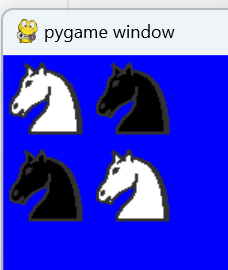
\includegraphics[width=0.4\textwidth,keepaspectratio]{img/e2a.png}\\
			\hline
			%%%%%%%%%%%%			
		\end{tabular}
	\end{table}
	%%%%%%%%%%%%%%%%%%%%%%%%
	\begin{table}[H]
		\begin{tabular}{|c|}
			\hline 
			\rowcolor{tablebackground}
			\color{white}\textbf{LECCIONES APRENDIDAS Y CONCLUSIONES}  \\
			\hline 
			\textbf{aqui ira la LECCIONES APRENDIDAS Y CONCLUSIONES}  \\
			\hline 
			%%%%%%%%%%%%
			\rowcolor{tablebackground}
			\color{white}\textbf{REFERENCIAS Y BIBLIOGRAFÍA}  \\
			\hline 
			\textbf{aqui ira la REFERENCIAS Y BIBLIOGRAFÍA}  \\
			\hline 
			%%%%%%%%%%%%			
		\end{tabular}
	\end{table}
	%%%%%%%%%%%%%%%%%%%%%%%%
	\subsection{USAR COMO GUIA PARA EL INFORME}
	\begin{itemize}	
		\item Se tuvieron que implementar las funciones negative, join y under. 
		En el codigo se detalla lo que hacen.
	\end{itemize}
	\lstinputlisting[language=Python, caption={Picture version 1},numbers=left,]{src/pic01.py}
	Para implementar el negativo se cambia el color de cada carácter, a excepción del espacio
	ya que este no tiene inverso con doble for(1 anidado). Juntando estos caracteres
	por medio en una cadena y despues juntando esta cadena al nuevo arreglo 
	con el metodo append.
	\lstinputlisting[language=Python, caption={Ejercicio 2 a},numbers=left,]{src/e2a.py}
	Para poder hacer que se dibuje como se mostrara el la figura de abajo se tuvo de juntar un caballo
	blanco con uno negro en la primera fila; para ello se utilizo join y negative. Para la segunda
	fila se necesito saltar a la siguiente fila por lo que se utilizo el metodo under.
	\begin{figure}[H]
		\centering
		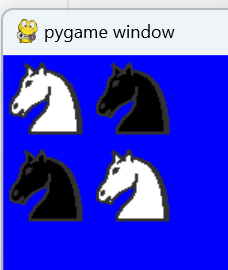
\includegraphics[width=0.4\textwidth,keepaspectratio]{img/e2a.png}
		\caption{Ejecución exitosa ejercicio 2 a}
	\end{figure}
	%%%%%%%%%%%%%%%%%%%%%%%%%%%%%
\subsection{Pregunta: Explique: ¿Para qué sirve el directorio pycache?}
\begin{itemize}
	\item Sirve para guardar los compilados de python, asi como en java al ejecutarlos se crean
	los .class en python se crean los .pyc. Esto se hace automaticamente ya que se importan 
	modulos de otras clases como se da en este caso.
\end{itemize}
	\clearpage	
\end{document}